\section{Trabajo top}

%-----------------------    ---------------------------------

\begin{frame}
\frametitle{¿Qué es un trabajo \emph{bueno}?}

\begin{itemize}
   \item Un trabajo que te permita ser creativo
   \item Un trabajo donde trabajes con últimas tecnologías
   \item Un trabajo donde puedas ascender sin dejar de ser ingeniero
   \item Un trabajo donde te paguen bien (y otros beneficios)
\end{itemize}

Hay muchas empresas donde buscan este tipo de perfil: Google, Apple, Facebook,
Microsoft, Yahoo!, Amazon...

\end{frame}

%-----------------------    ---------------------------------

\begin{frame}
\frametitle{Salarios en las compañías top}

\begin{center}
  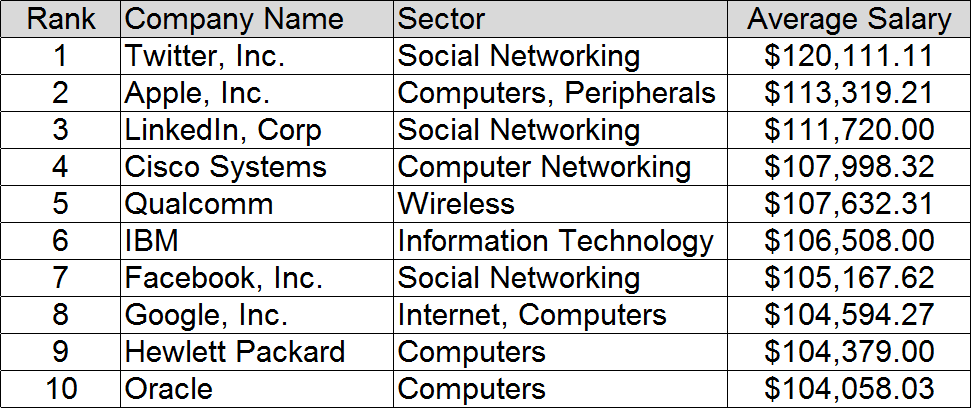
\includegraphics[width=10cm]{figs/toppaytech.png}
\end{center}


\begin{flushright}
{\tiny
http://img59.imageshack.us/img59/802/toppaytech.png
}
\end{flushright}

\end{frame}


%-----------------------    ---------------------------------

\begin{frame}
\frametitle{¿Qué te piden en estos trabajos?}

\begin{itemize}
   \item Estructuras de datos
   \item Algoritmia
   \item Experiencia en programación
   \item Redes de ordenadores
   \item Sistemas operativos
\end{itemize}

\end{frame}


%-----------------------    ---------------------------------

\begin{frame}
\frametitle{Más lecturas}

\begin{itemize}
   \item Hay varios libros sobre este tema, algunos en la biblioteca:
   \begin{itemize}
     \item Cracking the coding interview: 150 programming interview questions and solutions
     \item The Google Interview
     \item Elements of Programming Interviews: The Insiders' Guide
     \item Top 10 coding interview problems asked in Google with solutions: Algorithmic Approach
     \item Are You Smart Enough to Work at Google?: Fiendish Puzzles And Impossible Interview Questions From The World's Top Companies
     \item Get a Job WITHOUT an Interview - Google \& Beyond!: ``We don't mind to lose a good applicant, but definitely not hire a bad applicant.''
     \item The Google Resume: How to Prepare for a Career and Land a Job at Apple, Microsoft, Google, or any Top Tech Company
   \end{itemize}
\end{itemize}

\end{frame}



